\documentclass[11pt,twoside,a4paper]{book}  
% definice dokumentu
\usepackage[czech, english]{babel}
\usepackage[T1]{fontenc} 				% pouzije EC fonty 
\usepackage[utf8]{inputenc} 			% utf8 kódování vstupu 
\usepackage[square, numbers]{natbib}	% sazba pouzite literatury
\usepackage{indentfirst} 				% 1. odstavec jako v cestine, pro práci v aj možno zakomentovat
\usepackage{fancyhdr}					% tisk hlaviček a patiček stránek
\usepackage{nomencl} 					% umožňuje snadno definovat zkratky a jejich seznam

%%%%%%%%%%%%%%%%%%%%%%%%%%%%%%%%%%%%%%%%%%%%%%%%%%%%%%%%%%%%%%%
% informace o práci
\newcommand\WorkTitle{Nástroj pro tvorbu a sdílení HTML5 prezentací na webu}		% název
\newcommand\FirstandFamilyName{Radek Ježdík}															% autor
\newcommand\Supervisor{Ing. Ondřej Macek}															% vedoucí

\newcommand\TypeOfWork{Bakalářská práce}	% typ práce [Diplomová práce | Bakalářská práce | Bachelor's Project | Master's Thesis ]	

% Nastavte následují podle vašeho oboru a programu (pomoc hledejte na http://www.fel.cvut.cz/cz/education/bk/prehled.html)								
\newcommand\StudProgram{Softwarové technologie a management, Bakalářský}	% program
\newcommand\StudBranch{Softwarové inženýrství}           					% obor

%%%%%%%%%%%%%%%%%%%%%%%%%%%%%%%%%%%%%%%%%%%%%%%%%%%%%%%%%%%%%%%
% minimální importy
\usepackage{graphicx}					% pro vkládání obrázků
\usepackage{k336_thesis_macros} 		% specialni makra pro formatovani DP a BP
\usepackage[
pdftitle={\WorkTitle},				% nastaví v informacích o pdf název
pdfauthor={\FirstandFamilyName},	% nastaví v informacích o pdf autora
colorlinks=true,					% před tiskem doporučujeme nastavit na false, aby odkazy a url nebyly šedé při ČB tisku
breaklinks=true,
urlcolor=red,
citecolor=blue,
linkcolor=blue,
unicode=true,
]
{hyperref}								% pro zobrazování "prokliknutelných" linků 

% rozšiřující importy
\usepackage{listings} 			%slouží pro tisk zdrojových kódů se syntax higlighting
\usepackage{algorithmicx} 		%slouží pro zápis algoritmů
\usepackage{algpseudocode} 		%slouží pro výpis pseudokódu
\usepackage{enumitem}

%%%%%%%%%%%%%%%%%%%%%%%%%%%%%%%%%%%%%%%%%%%%%%%%%%%%%%%%%%%%%%%
% příkazy šablony
\makenomenclature								% při překladu zajistí vytvoření pracovního souboru se seznamem zkratek

\let\oldUrl\url									% url adresy budou zobrazeny: <url> 
\renewcommand\url[1]{<\texttt{\oldUrl{#1}}>}

%%%%%%%%%%%%%%%%%%%%%%%%%%%%%%%%%%%%%%%%%%%%%%%%%%%%%%%%%%%%%%%
% vaše vlastní příkazy
\newcommand*{\nomExpl}[2]{#2 (#1)\nomenclature{#1}{#2}} 	% usnadňuje zápis zkratek : Slova ke Zkrácení (SZ)
\newcommand*{\nom}[2]{#1 \nomenclature{#1}{#2}} 			% usnadňuje zápis zkratek : SZ


\usepackage{nameref}


\lstset{
	literate=%
		{á}{{\'a}}1
		{í}{{\'i}}1
		{é}{{\'e}}1
		{ý}{{\'y}}1
		{ú}{{\'u}}1
		{ó}{{\'o}}1
		{ě}{{\v{e}}}1
		{š}{{\v{s}}}1
		{č}{{\v{c}}}1
		{ř}{{\v{r}}}1
		{ž}{{\v{z}}}1
		{ď}{{\v{d}}}1
		{ť}{{\v{t}}}1
		{ň}{{\v{n}}}1
		{ů}{{\r{u}}}1
		{Á}{{\'A}}1
		{Í}{{\'I}}1
		{É}{{\'E}}1
		{Ý}{{\'Y}}1
		{Ú}{{\'U}}1
		{Ó}{{\'O}}1
		{Ě}{{\v{E}}}1
		{Š}{{\v{S}}}1
		{Č}{{\v{C}}}1
		{Ř}{{\v{R}}}1
		{Ž}{{\v{Z}}}1
		{Ď}{{\v{D}}}1
		{Ť}{{\v{T}}}1
		{Ň}{{\v{N}}}1
		{Ů}{{\r{U}}}1
}
\lstset{basicstyle=\ttfamily}

%%%%%%%%%%%%%%%%%%%%%%%%%%%%%%%%%%%%%%%%%%%%%%%%%%%%%%%%%%%%%%%
% vlastní dokument
%%%%%%%%%%%%%%%%%%%%%%%%%%%%%%%%%%%%%%%%%%%%%%%%%%%%%%%%%%%%%%%
\begin{document}
	
	%%%%%%%%%%%%%%%%%%%%%%%%%% 
	% nastavení jazyka, kterým je práce psána
	\selectlanguage{czech}	% podle jazyka práce nastavte na [czech | english]
	\translate				% nastaví české nebo anglické popisy (např. katedra -> department); viz k336_thesis_macros

	%%%%%%%%%%%%%%%%%%%%%%%%%%    
	% Poznamky ke kompletaci prace
	% Nasledujici pasaz uzavrenou v {} ve sve praci samozrejme 
	% zakomentujte nebo odstrante. 
	% Ve vysledne svazane praci bude nahrazena skutecnym 
	% oficialnim zadanim vasi prace.
	{
	\pagenumbering{roman} \cleardoublepage \thispagestyle{empty}
	\chapter*{Zadání projektu}
	Vytvořte nástroj pro tvorbu a sdílení HTML5 prezentací na webu. Webový backend umožní  tvorbu a editaci slidů a jejich sdílení. Pro prezentaci použijte vhodnou JavaScriptovou knihovnu, kterou rozšiřte o možnost testování čtenářů prezentace. Další požadavky na software sesbírejte na základě vytvořeného prototypu.\\\\
	
	\noindent Očekávaný výstup aplikace:
	\begin{enumerate}
		\item Analýza, návrh a implementace webové aplikace pro tvorbu, editaci a sdílení prezentací
		\item Rozšíření prezentační JS knihovny
		\item Nasazení a otestování aplikace
	\end{enumerate}
	\newpage
	}

	%%%%%%%%%%%%%%%%%%%%%%%%%%    
	% Titulni stranka / Title page 
	\coverpagestarts

	%%%%%%%%%%%%%%%%%%%%%%%%%%%    
	% Poděkovani / Acknowledgements 

	\acknowledgements
	\noindent
	Zde můžete napsat své poděkování, pokud chcete a máte komu děkovat.


	%%%%%%%%%%%%%%%%%%%%%%%%%%%   
	% Prohlášení / Declaration 

	\declaration{V~Praze dne 7.\,1.\,2013}
	%\declaration{In Kořenovice nad Bečvárkou on May 15, 2008}


	%%%%%%%%%%%%%%%%%%%%%%%%%%%%    
	% Abstrakt / Abstract 
 
	\abstractpage

	Translation of Czech abstract into English.

	% Prace v cestine musi krome abstraktu v anglictine obsahovat i
	% abstrakt v cestine.
	\vglue60mm

	\noindent{\Huge \textbf{Abstrakt}}
	\vskip 2.75\baselineskip

	\noindent
	TODO Obsahem by mělo být: řeším takový a takový problém v práci se dozvíte to a to. (ne shrnutí zadání)

	%%%%%%%%%%%%%%%%%%%%%%%%%%    
	% obsahy a seznamy
	\tableofcontents		% Obsah / Table of Contents 

	% pokud v práci nejsou obrázky nebo tabulky - odstraňte jejich seznam
	\listoffigures			% Obsah / Table of Contents 
	% \listoftables			% Seznam tabulek / List of Tables

	%%%%%%%%%%%%%%%%%%%%%%%%%% 
	% začátek textu  
	\mainbodystarts



\chapter{Úvod}
Tento projekt má za cíl vytvořit webový portál, který uživatelům umožní nejen snadné sdílení vlastních prezentací, ale také jejich tvorbu. Jediným nástrojem tak uživatel prezentaci vytvoří a poté ji v rámci portálu či jiných komunikačních kanálů, jako jsou sociální sítě, může šířit dál mezi lidi. Prezentace by se měly zaměřovat na podání informací a na případné testování uživatelů z nově nabytých vědomostí. Portál tak bude sloužit jak přednášejícím, tak posluchačům či žákům.

\section{Cíle}
Sdílení a tvorba prezentací online není originální myšlenka a v současné době existuje řada známých i méně známých portálů, které v této oblasti dosáhly dobrých výsledků. Proto jsem se rozhodl projekt zaměřit zejména na použití ve vzdělávacích institucích či školách a nebo na odborných konferencích, kde je důležité v prezentacích podat důležité informace, nejen tedy hlavní body.

Stejně tak je důležité, aby tyto prezentace byly použitelné i mimo přednášku, tedy aby podaly významné informace i bez mluveného slova, například pro domácí přípravu nebo vlastní rozvoj. Pro zjednodušení tohoto cíle proto nástroj bude poskytovat několik prostředků jako je zvýraznění kódu programovacích jazyků či zobrazení matematických vzorců pomocí syntaxe \LaTeX. Navíc bude možné do prezentací vkládat kontrolní otázky, na které budou moci uživatelé odpovídat a systém je opraví, případně lze přidat i odkazy na snímek, ve kterém se o otázce mluví.

\section{Příležitosti}
Od práce na tomto projektu si slibuji větší porozumění technologiím HTML5 a JavaScriptu. Zajímavou příležitostí je tedy vyzkoušení si tvorby webových stránek, které nejsou jen dalším typickým informačním systémem. V tomto projektu lze najít spoustu problémů a nových a zajímavých technologií, na kterých si vyzkouším vývoj nových klientských aplikací.






\chapter{Analýza}
V této kapitole je čtenář uveden do problematiky \nom{HTML}{HyperText Markup Language} prezentací. Dále jsou porovnávány vybrané knihovny, které zajišťují funkčnost HTML prezentací. Nakonec je představena vize vyvíjeného systému a porovnání s podobnými již existujícími systémy.

\section{Popis problému, cíle}
Cílem projektu je vytvořit webový nástroj pro tvorbu, úpravu a sdílení prezentací založených na technologii HTML5.

V současné době se většina aplikací, nástrojů a služeb přesouvá na internet, kde se mimo jiné klade důraz na sdílení mezi uživateli. Prezentace nejsou výjimkou a na trhu lze najít již několik zavedených služeb, které se tvorbou a sdílením prezentací zabývají (více na str. \pageref{chap:existujiciSystemy}). S příchodem HTML5 a CSS3\footnote{V době psaní této práce bylo HTML5 ve stádiu návrhu organizací W3C. \cite{html5-2014}} se objevily knihovny, které využívají těchto nových technologií pro zobrazení webových prezentací přímo v prohlížeči bez doplňků třetích stran. 



\section{HTML5 prezentace}
Prezentace založené na HTML jsou z pohledu kódu běžná webová HTML stránka. K~popisu obsahu snímků se používají sémantické značky běžně používané v HTML (např. nadpisy, odstavce, obrázky). Pro úpravu grafické podoby se používá CSS. K~oživení takovéto stránky a~vytvoření dojmu prezentace a přechodů mezi snímky se používá JavaScript. Funkčnost prezentace tedy zajišťují JavaScriptové knihovny.

Každá z existujících knihoven používá jiná pravidla pro konfiguraci prezentace či jednotlivých snímků. Následující výpis ukazuje zdrojový kód jednoduché HTML prezentace při použití knihovny Deck.js.

\begin{lstlisting}[caption=Ukázka zdrojového kódu HTML prezentace (Deck.js)]
<article class="deck-container">
  <section class="slide">
    <h1>Moje prezentace</h1>
  </section>

  <section class="slide">
    <h2>Nadpis snímku</h2>
    <p>Osnova:</p>
    <ul>
      <li>Bod 1</li>
      <li>Bod 2</li>
      <li>Bod 3</li>
    </ul>
  </section>
</body>
\end{lstlisting}

Zobrazení právě jednoho snímku, přecházení mezi snímky a držení stavu prezentace pak obstarává knihovna samotná. Na autorovi prezentace je jen napsat obsah snímků a dodržet konvence požadované knihovnou.


\section{Výběr JavaScriptové knihovny}
Knihoven pro zobrazení prezentací založených na technologii (X)HTML bylo vytvořeno celá řada (viz \cite{htmlslideshowweb}). Většina z nich je ovšem už zastaralá, nefunkční nebo neodpovídající požadovaným kvalitám, například použitelnosti, uživatelské či implementační, nebo vzhledu. Následující seznam uvádí několik zdařilých knihoven, které se objevily po uvedení podpory HTML5 v~prohlížečích.

\begin{itemize}
	\item reveal.js
	\item impress.js
	\item Google I/O HTML5 slide template
	\item deck.js
\end{itemize}


\subsection{Reveal.js} \label{chap:revealjs}
Reveal.js\footnote{\url{https://github.com/hakimel/reveal.js/}} podporuje kromě posunu snímků horizontálně také vnořené snímky, na které se lze dostat posunem dolů. Má několik zajímavých rozšíření, např. podpora syntaxe Markdown pro psaní obsahu a barevné zvýraznění kódu programovacích jazyků pomocí knihovny highlight.js. V novém okně pak umožňuje zobrazit aktuální a následující snímek včetně poznámek přednášejícího.

\subsection{Impress.js}
Impress.js\footnote{\url{https://github.com/bartaz/impress.js/}} se více zaměřuje na vizuální jedinečnost prezentace. Dosahuje toho složitými transformacemi přechodů mezi snímky. Ty jsou rozloženy v~prostoru, a to nejen ve 2D ale i ve 3D, o různých velikostech a při přechodu mezi snímky se pohled působivě otáčí a přesouvá.

Nevýhoda této knihovny je právě v tomto jednoúčelově pojatému zobrazení. Pro účely tohoto projektu je tak knihovna až moc složitá, hlavně kvůli určení pozic snímků a transformací, a pro informativní prezentace se příliš nehodí - přechody mezi snímky spíše vyrušují.

\subsection{Google I/O HTML5 slide template}
HTML5 šablonu od Googlu\footnote{\url{https://code.google.com/p/io-2012-slides/}} používají při svých prezentacích vývojáři na konferencích Google I/O. Knihovna je proto v dobré kvalitě a velmi dobře uzpůsobená pro přednášející. Obsahuje tzv. prezentační mód podobný tomu v reveal.js. Poskytuje také zvýraznění kódu programovacích jazyků a to včetně možnosti zdůraznit jen určitou část kódu, které se přednášející chce věnovat podrobněji.

Knihovna ovšem nenabízí žádnou dokumentaci a tak snižuje možnost na další rozšíření. Dále má prezentace pevnou velikost a tak na menších displejích či oknech jsou snímky oříznuté. Nevýhodou je také o něco složitější konfigurace.

\subsection{Deck.js}
Knihovna deck.js\footnote{\url{https://github.com/imakewebthings/deck.js}} je v základu o něco jednodušší než ostatní knihovny výše. Je napsaná v jQuery, je velmi dobře zdokumentovaná a rozšiřitelná. Existuje pro ni řada pluginů, například již zmíněný prezentační mód či podpora Markdown syntaxe pro popis snímků.

\subsection{Zhodnocení}
Pro účely tohoto projektu byla použita knihovna deck.js, která je o něco jednodušší. Líbí se mi více celkový vzhled a jednoduchost a to, že je postavena na jQuery. Případně lze také využít existujících rozšíření nebo vytvořit vlastní. Knihovna reveal.js ovšem urazila během práce na tomto projektu velký kus cesty a v současné době je asi nejvíce rozšířenou a používanou knihovnou pro HTML prezentace. O knihovně byla také napsána výuková kniha \cite{howtobook}.


\section{Webový portál}
Pro uživatele má portál sloužit jako prostředník pro sdílení prezentací – ať už v~rámci portálu mezi jeho uživateli nebo
posíláním URL odkazů na prezentace v~emailech, příspěvcích na sociálních sítích Facebook nebo Twitter a dalších. V principu se tak bude podobat portálům jako YouTube, SlideShare nebo GitHub, které se zaměřují na vystavení vlastní tvorby (videí, prezentací, kódu) a její sdílení.

Sdílení prostřednictvím webového portálu je dvojího typu. Uživatelé mohou sledovat jiné uživatele a o aktivitách těchto sledovaných uživatelů, například publikace nové prezentace, bude snadněji upozorněn. Druhý typ je pak sdílení opačným směrem, od autora prezentace uživatelům portálu. Uživatele si autor vybere podle uživatelského jména či e-mailu.

Důležitá je také zpětná vazba od uživatelů prohlížející si prezentace. Řešením je možnost uživatelů přidávat komentáře k jednotlivým prezentacím.

\section{Editor}
Důležitou částí tohoto projektu je editor pro úpravy prezentace. Protože obsah prezentace je tvořen pomocí HTML, nabízí se
několik možností, jak editaci pojmout:

\begin{enumerate}
	\item psaním samotného HTML kódu.
	\item využitím editoru typu \nom{WYSIWYG}{What You See Is What You Get}.
	\item využitím jednoduchého textového značkovacího jazyka (lightweight markup language).
\end{enumerate}

Psaní samotného HTML kódu bylo vyloučeno bez většího váhání. HTML není nijak úsporný značkovací jazyk a pro uživatele, kteří neznají HTML, by byl překážkou. Na druhou stranu ale poskytuje největší možnou kontrolu nad podobou a funkčností prezentace. Kdyby ovšem editor měl být založen pouze na psaní HTML kódu, nebyl by vůbec potřeba - pro většinu uživatelů by pak bylo výhodnější použít nástroje, na které jsou zvyklí, a pak pouze nahrát hotovou prezentaci na web.

Editor WYSIWYG je koncept dobře známý z desktopových aplikací. Jedná se o přímou úpravu obsahu a uživatel nepřichází do styku se zdrojovým kódem. Jeho největší výhodou je pak jednoduchost pro uživatele, kteří výsledek svých úprav vidí okamžitě. Ve webovém prostředí se používá pro jednoduché vytváření stránek, například v CMS systémech. Nevýhodou je, že neexistuje standard, který by dodržovaly všechny prohlížeče. Poskytuje také menší kontrolu nad výsledným kódem. 

Vybrána byla nakonec poslední možnost - jednoduchý textový značkovací jazyk, jímž se bude popisovat obsah snímku. Zdrojový text se následně převádí do kódu HTML. Více je popsáno v~kapitole \ref{chap:realizace} \nameref{chap:realizace} na str. \pageref{chap:realizace}.

\section{Prohlížení prezentace}
Zajímavou vlastností, která se liší od ostatních webových služeb pro prohlížení prezentací, byla možnost poskytnout větší interaktivitu s uživatelem. Protože je prezentace běžná HTML stránka, lze využít možností webových technologií pro vytvoření nových vlastností prezentace.

Jednou z nich je možnost odpovídat na otázky a kontrolovat správné odpovědi přímo v prezentaci. Uživatelé si pak mohou vyzkoušet, co se z prezentace naučili. Navíc je možné zobrazit doplňkový text při správné či špatné odpovědi. Ten pak může obsahovat nejen vysvětlení správné odpovědi, ale třeba i odkaz na snímek týkající se dané otázky.


\section{User stories}\label{chap:userstory}
Následující odstavce popisují uživatelské role, které se při používání systému objevují. Každá role pak má nějaké práva či možnosti využití systému. Popis je zapsán pomocí techniky zvané user story používané v agilních metodikách vývoje software. \\\\

\noindent \textbf{Nepřihlášený uživatel} bude mít možnost:
\begin{enumerate}
	\item \textbf{prohlížet veřejně dostupné prezentace}, k~tomu použije 
		\begin{enumerate}[label*=\arabic*.]
			\item vyhledávací formulář na webu.
			\item adresu URL na stránku s prezentací, kterou dostane jiným komunikačním kanálem.
		\end{enumerate}
	\item \textbf{vyhledat prezentace} vyhledávacím formulářem podle názvu nebo autora, aby mohl
		\begin{enumerate}[label*=\arabic*.]
			\item zhlédnout hledanou prezentaci.
			\item číst komentáře pod prezentací.
			\item zobrazit prezentace hledaného uživatele.
		\end{enumerate}
	\item \textbf{přihlásit se} do systému pomocí přihlašovacího formuláře, aby získal oprávnění přihlášeného uživatele (viz níže).
	\item \textbf{registrovat se} do systému pomocí registračního formuláře, aby se mohl přihlásit.
\end{enumerate}


\noindent \textbf{Přihlášený uživatel} bude mít možnost:
\begin{enumerate}
	\item \textbf{vytvářet} prezentace pomocí editoru prezentací.
	\item \textbf{posílat komentáře} k~prezentacím, ke kterým má přístup, pomocí formuláře pod prezentací.
	\item \textbf{prohlížet veřejné a jemu sdílené} prezentace.
	\item \textbf{vyhledat prezentace} vyhledávacím formulářem podle názvu nebo autora, aby kromě toho co může nepřihlášený uživatel:
		\begin{enumerate}[label*=\arabic*.]
		\item \textbf{sledovat nebo zrušit sledování} hledaného uživatele.
		\end{enumerate}
	\item \textbf{vidět seznam jemu sdílených prezentací}.
	\item \textbf{vidět seznam veřejných prezentací} uživatelů, které \textbf{sleduje}.
	\item \textbf{změnit své heslo}.
	\item \textbf{odhlásit se}.
\end{enumerate}


\noindent \textbf{Autor prezentace} bude mít možnost:
\begin{enumerate}
	\item \textbf{upravit prezentaci} v~editoru, aby ji o něco doplnil nebo ji opravil.
	\item \textbf{smazat prezentaci}.
	\item \textbf{smazat jakýkoliv komentář} k~vlastní prezentaci.
	\item \textbf{sdílet prezentaci} ostatním uživatelům portálu.
\end{enumerate}


\noindent \textbf{Autor komentáře} bude mít možnost:
\begin{enumerate}
	\item smazat svůj komentář.
\end{enumerate}


\section{Nefunkční požadavky}
\begin{enumerate}
	\item Systém bude přístupný přes webové rozhraní.
	\item Systém bude pro uživatele nezávislý na platformě.
	\item Systém bude využívat technologii HTML5.
	\item Pro prezentace bude systém využívat JavaScriptovou knihovnu.
\end{enumerate}


\section{Rešerše existujících řešení} \label{chap:existujiciSystemy}
Během analýzy byly také vyhledány a vyzkoušeny již existující služby, jejichž funkčnost se nejvíce podobá zadání tohoto projektu. Následující odstavce popisují jejich funkci a rozdíly.


\subsection{SlideShare}
SlideShare\footnote{\url{http://www.slideshare.net}} je na internetu velmi známý webový portál pro sdílení prezentací. Obsahuje podobné mechanismy sdílení a zpětné vazby a umožňuje prezentace umisťovat na jiné stránky (tzv. embedded presentace). Prezentace jsou ovšem velmi statické – bez animací a bez větší interaktivity s~uživatelem. Některé prezentace jsou jen obrázkové, nejde tedy označit text ani následovat odkaz. Největší nevýhodou je, že prezentace nelze na portálu přímo tvořit, lze je pouze nahrávat ve formátech PDF, PPT a dalších z~lokálního úložiště. Jakákoliv změna v~prezentaci se tak musí nahrát znovu.

\subsection{Prezi}
Prezi\footnote{\url{http://www.prezi.com}} funguje na podobném principu jako SlideShare, ale zaměřuje se daleko více na grafickou stránku a zakládá si na kreativitě uživatelů a vyjádření jejich idejí pomocí celkového vzhledu prezentace. Prezentace se značně liší od běžných prezentací, které známe například z~Microsoft PowerPoint. Jejich použití se hodí hlavně pro vyjádření nějaké myšlenky či vize, méně se hodí pro podání důležitých informací. Pro zobrazení prezentace používá technologii Flash.

\subsection{Rvl.io}
Rvl.io\footnote{\url{http://www.rvl.io}} je služba od autora knihovny reveal.js popsané na str. \pageref{chap:revealjs}, kterou také používá pro zobrazení prezentací. Služba umožňuje sdílení i tvorbu prezentací přímo na webu. Sdílení je založeno na předávání adresy URL, poskytuje ale také vkládání prezentace do jiných stránek, podobně jako SlideShare. Pro úpravu prezentací využívá WYSIWYG editor, který ale poskytuje jen nezbytné minimum funkcí. Tento portál je velmi mladý a uveden byl po měsíci od započetí práce na tomto projektu. Služba byla v~době psaní této práce stále ve fázi beta testování.




\chapter{Návrh}

V následujícím textu bude čtenář seznámen s detailním návrhem systému. Kromě doménového modelu a popisu jednotlivých entit budou popsány použité technologie a knihovny.

\section{Doménový model}
\begin{figure}[ht]
	\begin{center}
		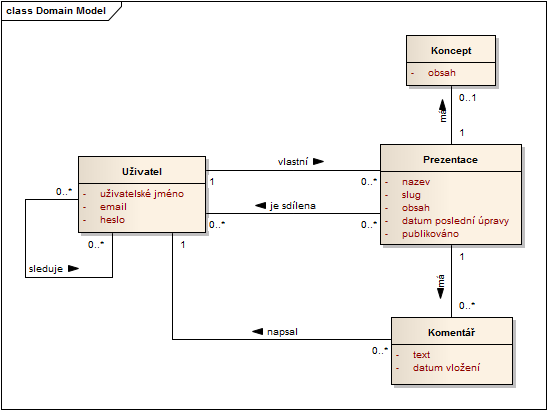
\includegraphics[width=14cm]{PRO-img/domain.png}
		\caption{Diagram doménového modelu}
		\label{fig:domainModel}
	\end{center}
\end{figure}

\subsection{Uživatel}
Uživatel představuje registrovaného uživatele systému. Registrovaný a přihlášený uživatel má výhody oproti nepřihlášenému (více na str. \pageref{chap:userstory}).

Pro úspěšnou registraci nového uživatele do systému musí nepřihlášený uživatel zadat:

\begin{itemize}
	\item \textbf{uživatelské jméno}, pod kterým se bude prezentovat a přihlašovat. Stejné uživatelské jméno musí být v systému registrováno jenom jednou.
	\item \textbf{e-mail}, který musí být v systému jedinečný.
	\item \textbf{heslo}, minimální délka 4 znaky.
\end{itemize}

Uživatelé se mohou navzájem tzv. sledovat. Uživatel je tak snadněji upozorněn na nové prezentace od sledovaných uživatelů.

\subsection{Prezentace}
Tato entita představuje jednu prezentaci, kterou uživatel pomocí systému vytvořil, tedy je jejím autorem. Má tyto povinné
vlastnosti:

\begin{itemize}
	\item \textbf{název}, pod kterým se daná prezentace bude zobrazovat ve výpisech.
	\item \textbf{slug} - zjednodušený název (malá písmena anglické abecedy, čísla a pomlčky), pod kterým bude prezentace dostupná přes adresu URL.
	\item \textbf{obsah}, jenž představuje složitější objekt textů jednotlivých snímků a různých nastavení prezentace.
\end{itemize}

Při vytvoření je prezentace ve stavu nepublikováno. Stav se změní na publikováno při publikaci prezentace v editoru. Pak je prezentace viditelná ostatním uživatelům v systému.

Prezentace může být sdílena konkrétním uživatelům portálu.


\subsection{Koncept}
Koncept je obsah prezentace (popis snímků, nastavení), který nebyl zatím publikován. Je viditelný pouze v editoru pro autora prezentace. Při publikaci změn prezentace se obsah konceptu překopíruje do obsahu vlastní entity prezentace.


\subsection{Komentář}
Komentář je uživatelem napsaná poznámka k dané prezentaci. Komentář může vkládat každý přihlášený uživatel. Povinné
vlastnostmi jsou:

\begin{itemize}
	\item \textbf{text komentáře} – obsah zprávy
	\item \textbf{datum a čas}, kdy byl komentář vložen
\end{itemize}

Komentář se váže k~jedné prezentaci a jednomu uživateli (autorovi komentáře).


\section{Serverová část}
Webový back-end jsem se rozhodl napsat v~programovacím jazyce PHP s~použitím českého webového aplikačního frameworku Nette\cite{nette}. Pro uchování dat byla použita databáze MySQL\cite{mysql}.

\subsection{Nette Framework}
Nette Framework je aplikační framework, který usnadňuje řešení mnoho problémů v oblasti webového vývoje v PHP. Implementuje návrhový vzor \nomExpl{MVP}{Model-View-Presenter} rozdělující aplikaci na logické vrstvy (viz níže). Běh aplikace je řízen událostmi, tedy využívá událostmi řízené programování. Dále obsahuje komponentový model zaměřený na znovupoužitelnost.

\subsection{MVP}
Návrhový vzor Model-View-Presenter řeší problém oddělení datové vrstvy, řízení událostí (např. od uživatele) a vykreslení daných dat\citep{mvp}. Následuje popis jednotlivých vrstev a jejich společné interakce.

\begin{itemize}
	\item Model - poskytuje rozhraní pro data určená k zobrazení
	\item View (pohled) - vykresluje data modelu a směruje uživatelské příkazy presenteru
	\item Presenter - prostředník mezi modelem a pohledem. Získává data z modelu a upravuje je pro zobrazení v pohledu. Řeší události vyvolané uživatelem.
\end{itemize}

\subsection{Architektura aplikační logiky}
Nette Framework ovšem neposkytuje žádné vlastní řešení modelové vrstvy a nechává tak programátorovi volné ruce na využití jiných knihoven nebo vlastních řešení zaměřujících se na obchodní a datovou logiku. Do presenteru je pak možné tyto služby předat pomocí návrhového vzoru Dependency injection\cite{di}.

Pro tento projekt byla využita databázová vrstva Nette\textbackslash{}Database, která poskytuje jednoduché rozhraní pro získávání dat z databáze. Komunikace s databází pak byla zabalena do repositářů, jenž poskytují metody pro navrácení jednotlivých entit a tvorbu a mazání záznamů. V případech, kdy je logika složitější a repositáře tuto funkčnost nemohou vykonat, je přidána další vrstva, fasáda. 

Lepší představu o průběhu chodu aplikace při uživatelském požadavku získáte z obrázku~\ref{fig:logika}. Všechny komponenty serverové části pak přehledně zobrazuje diagram balíčků~\ref{fig:balicky}.


\begin{figure}[ht]
	\begin{center}
		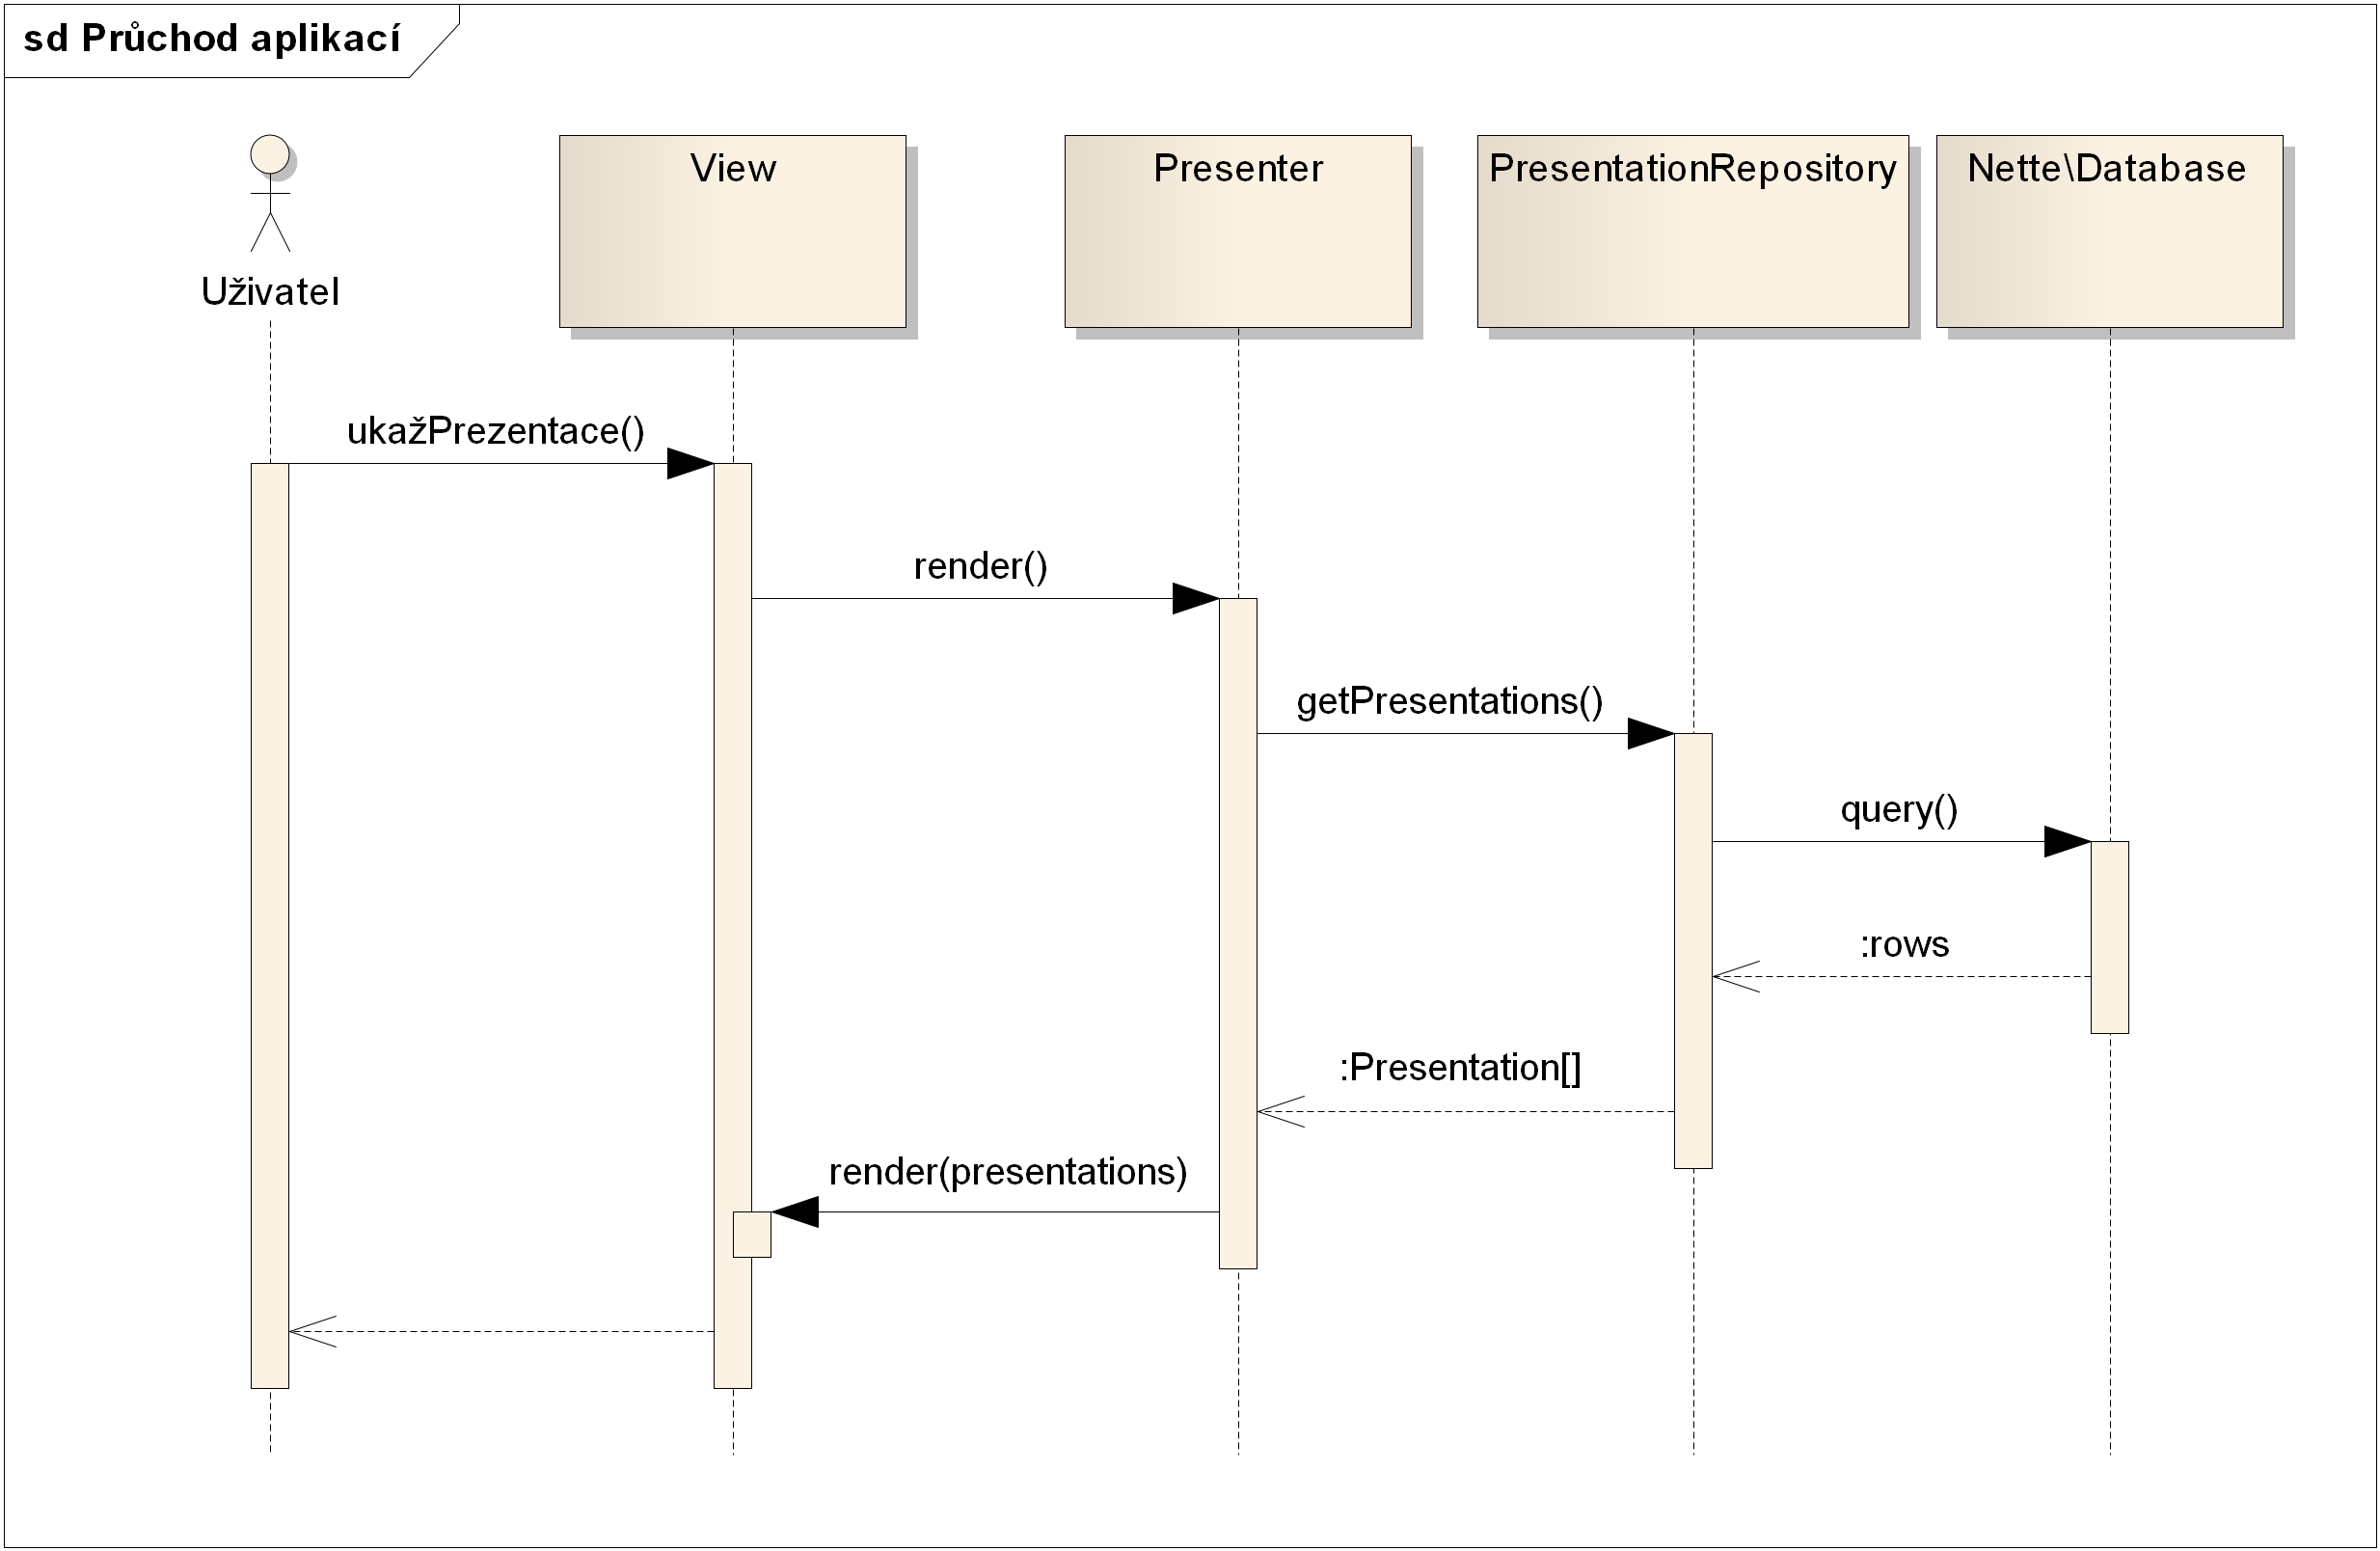
\includegraphics[width=14cm]{PRO-img/logika.png}
		\caption{Ukázka průchodu aplikace}
		\label{fig:logika}
	\end{center}
\end{figure}

\begin{figure}[ht]
	\begin{center}
		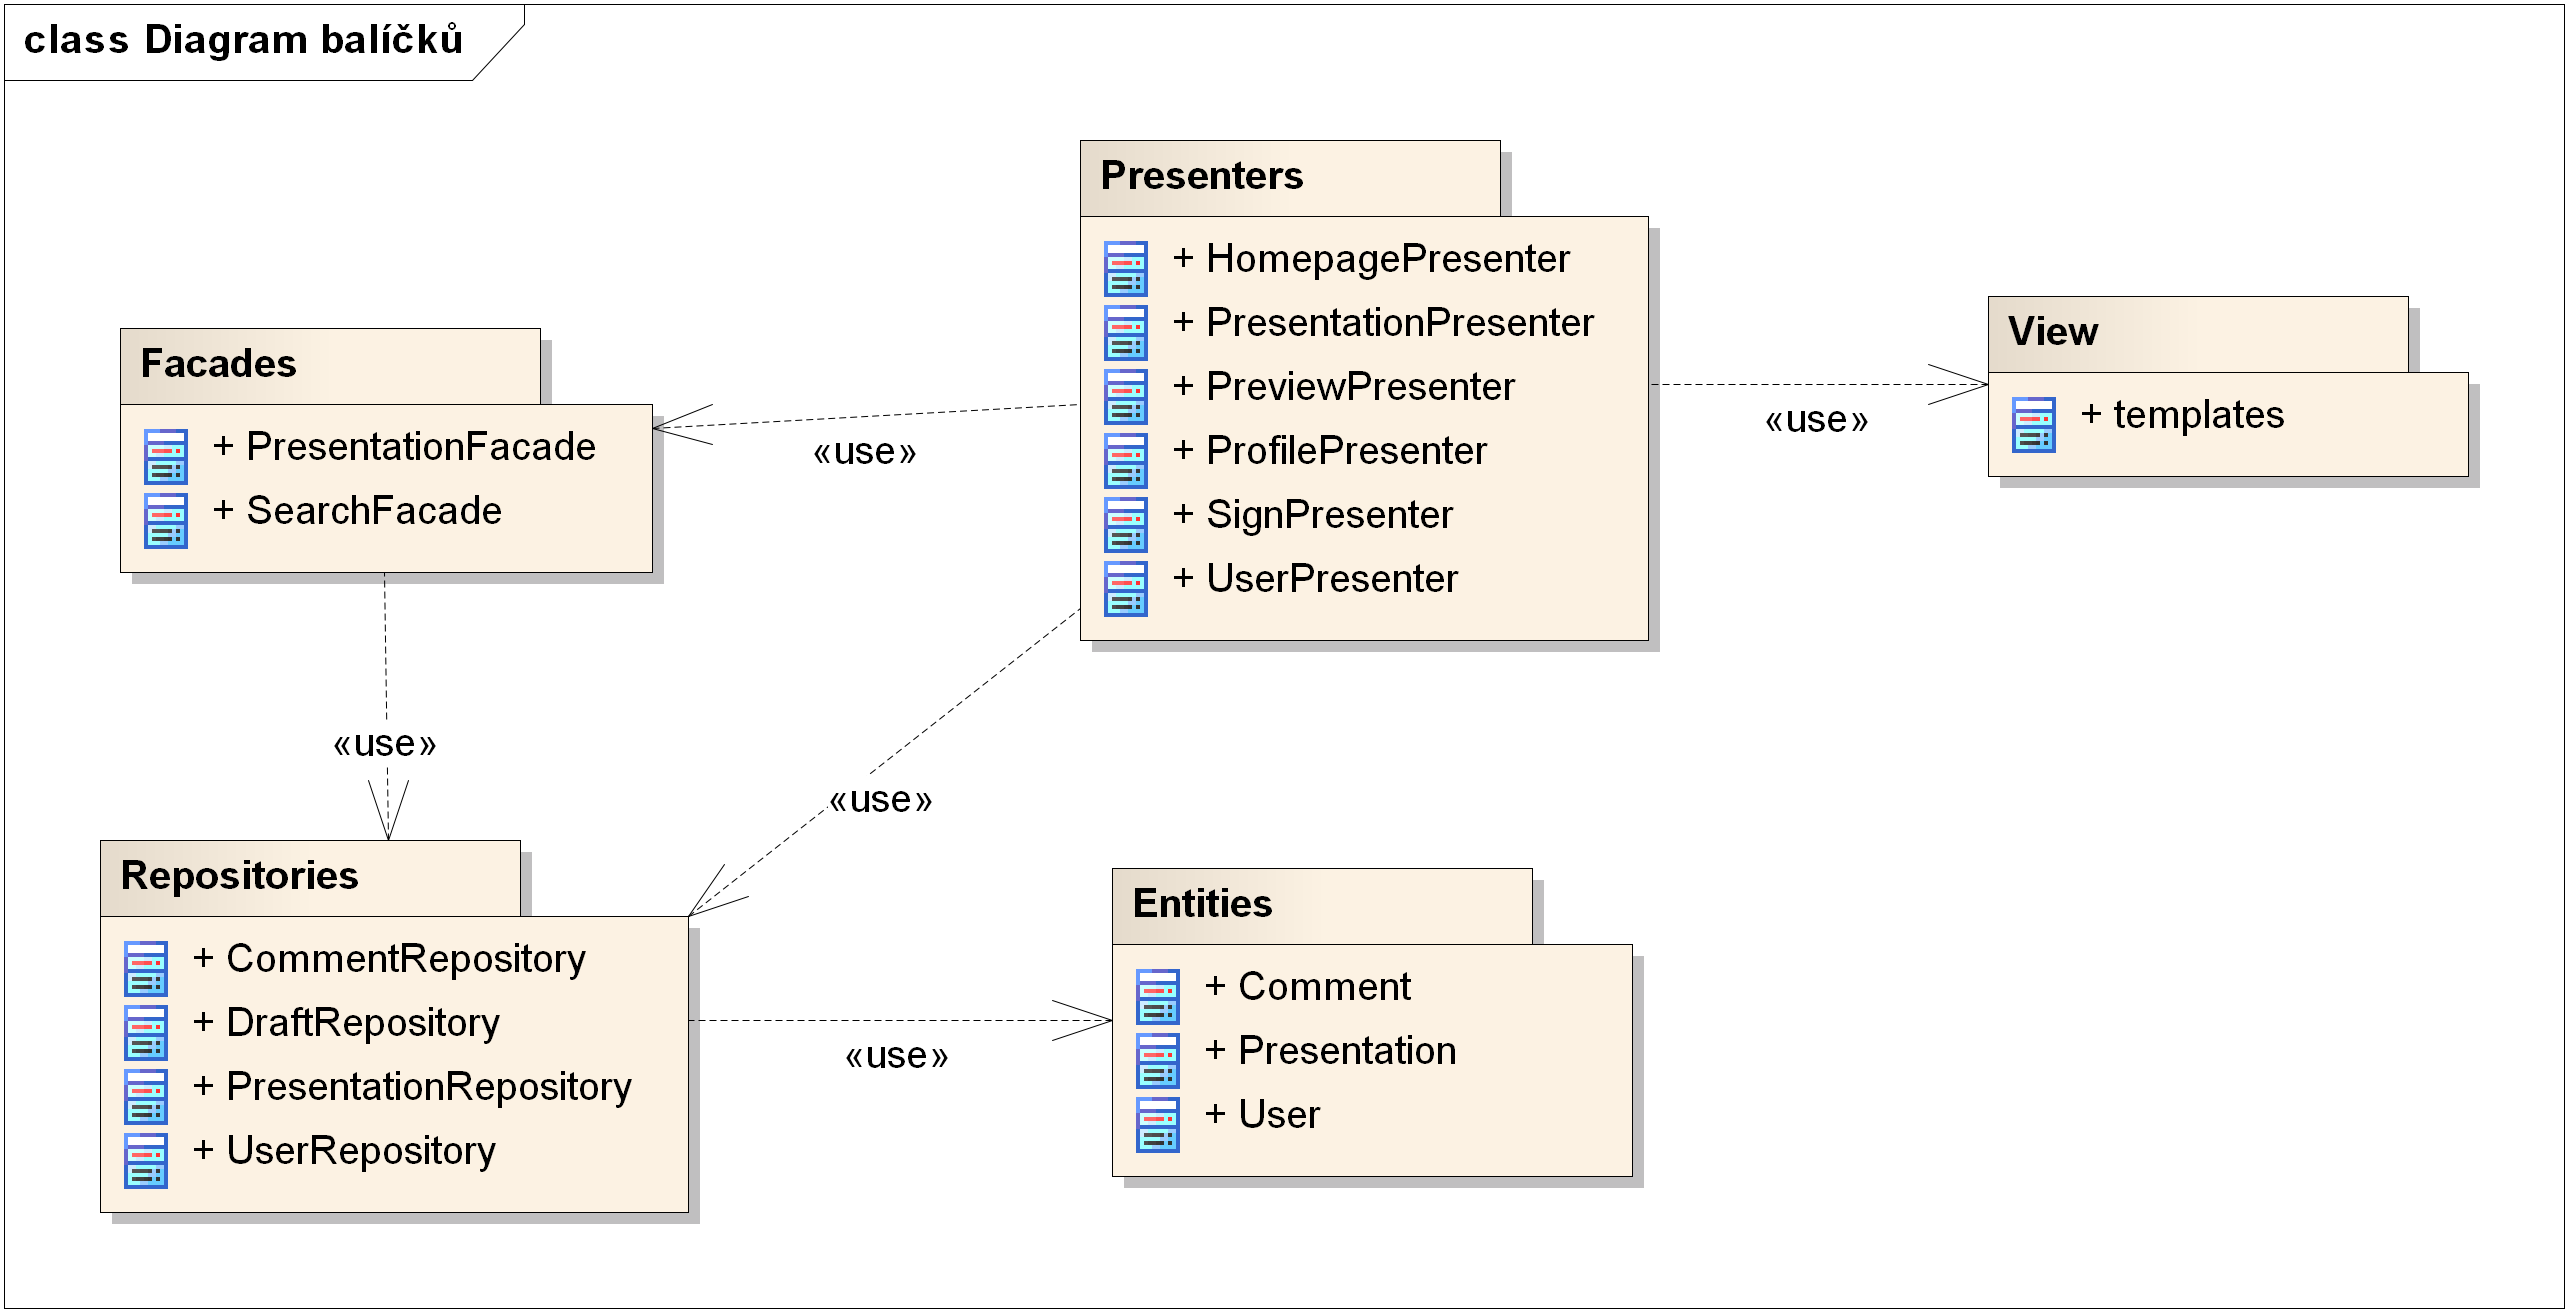
\includegraphics[width=14cm]{PRO-img/balicky.png}
		\caption{Diagram balíčků}
		\label{fig:balicky}
	\end{center}
\end{figure}


\section{Klientská část}
Na klientské prostředí jsou přenášeny výstupy v podobě HTML stránek. Pro jejich oživení a zlepšení uživatelské použitelnosti (např. klientské validace formulářů) se používá JavaScript. Vlastní kód byl však napsán v CoffeeScriptu\cite{coffee}, transkompilátoru, který se kompiluje do běžného JavaScriptu. 

Dále byla použita JavaScriptová knihovna jQuery\cite{jQuery}, která usnadňuje práci s HTML dokumentem a sjednocuje implementační rozdíly mezi prohlížeči.

Pro vzhled a grafické uživatelské rozhraní byl použit framework Bootstrap\cite{bootstrap}, který velmi usnadnil prototypování uživatelského rozhraní portálu bez nutnosti tvořit vzhled a ladit ho pro každý prohlížeč zvlášť. Dále poskytuje jednoduché metody pro tvorbu nabídek či zobrazení dialogových oken. Výhodou je i to, že Bootstrap poskytuje responsivní design a tak by se měl web chovat a zobrazovat dobře i na mobilních zařízeních.


\section{Editor}
Editoru prezentací byl přikládán větší význam, neboť bez této komponenty by systém nemohl realizovat myšlenku tohoto projektu. Značně se také liší od ostatních obyčejných webových stránek, jelikož se jedná z větší části o ryze klientskou jednostránkovou miniaplikaci.

Právě proto používá editor pár technologií navíc. Jako nejdůležitější se ukázalo použití JavaScriptového MVC frameworku AngularJS\cite{angular}. Jeho hlavní předností je dvoucestné provázání dat mezi pohledem (view) a modelem na straně klienta. Každá změna v~modelu se pak automaticky propaguje do pohledu a naopak. Snižuje se tak množství kódu, který otrocky nastavuje nebo zobrazuje data při jednotlivé změně. 

TODO wireframe editoru

Pro popis obsahu snímku, jak bylo zmíněno v analýze, byl se používá jednoduchý textový značkovací jazyk, který převádí text do HTML. Pro převod tohoto textu je použita PHP knihovna Texy!\cite{texy}, která implementuje vlastní stejnojmenný značkovací jazyk. Výhodou této knihovny je snadná rozšiřitelnost a také typografické úpravy výsledného textu. Více o výběru knihovny se dozvíte v~následující kapitole.

Součástí editoru je také panel nástrojů, který doplňuje textový vstup pro popis snímku. Uživateli ulehčí práci s psaním zdrojového~textu, například možností vložit značky pro tučné písmo či kurzívu atd. Pro panel nástrojů byla použita knihovna Texyla\cite{texyla}.



\chapter{Realizace klientské části} \label{chap:realizace}
V této kapitole se dozvíte o průběhu realizace klientské části aplikace, tj. editoru prezentací a zobrazení prezentací, co vedlo k rozhodnutím o podobě projektu a jaké problémy vyvstaly a jak byly řešeny.

\subsection{Prototyp editoru prezentací}
V~první fázi vývoje jsem se zabýval myšlenkou editoru prezentace jako hlavní komponenty, bez které by projekt neplnil požadovanou funkci. Následující text popisuje průběh práce na prototypu editoru prezentace.

\subsubsection{WYSIWYG editor}
Při prvním prototypování editoru snímků prezentace se počítalo s~použitím WYSIWYG editoru, tedy editoru, kde jsou změny vidět v reálném čase a uživatel při samotné úpravě snímků okamžitě vidí, jak bude vypadat konečný výsledek. Výhodou je, že uživatel nepotřebuje znát ani jazyk HTML (i když knihovny často poskytují i možnost kód HTML upravovat). Existuje mnoho knihoven, které WYSIWYG editor různě implementují. Protože ale neexistuje žádný standard, každý prohlížeč se chová trochu jinak a zároveň každá knihovna si různé věci implementuje po svém.

Nejdříve byla otestována WYSIWYG knihovna Aloha Editor\cite{aloha}, která se nejčastěji používá v \nom{CMS}{Content Management System} systémech. Nabízí několik zajímavých vlastností jako je např. repositář - prohlížeč obrázků, souborů či vlastních uživatelských objektů. Potíže ovšem nastaly se zobrazením panelu nástrojů a špatnou podporou CSS3 transformací, které jsou použity ve vzhledu deck.js prezentací. Největším problémem byla ovšem licence\footnote{pozn.: nedávno byla licence změněna na GPLv2, projekt byl ale už v tu dobu v pokročilé fázi vývoje}.

Jako další editor byl vyzkoušen Mercury Editor\cite{mercury}, který se zdál být vhodnější a komplexnější. I když se jedná o JavaScriptovou knihovnu, je vyvíjena v~Ruby pro použití v~Ruby On Rails aplikacích a tak bylo hodně věcí přizpůsobeno těmto technologiím (například počítala s~partial pohledy, které se posílají pomocí technologie \nom{AJAX}{Asynchronous JavaScript and XML} ze serveru). Nicméně knihovna není na jazyce Ruby závislá a lze ji použít bez něj.

Zde se ale po chvíli objevily problémy technického rázu – prohlížeče se právě díky neexistujícímu standardu chovaly rozdílně nebo se nechovaly podle očekávání. Výsledkem pak byl například špatný HTML kód nebo kód, který se už nedal nijak pomocí editoru opravit ani smazat. Jedním z~největších problémů bylo vkládání nového řádku. Prohlížeč někdy vložil značku odřádkování \verb|<br>| někdy nový odstavec \verb|<p>|. Chování tak nebylo předvídatelné. 

Objevily se i další chyby v~použitelnosti či bugy, na které jsem se pak snažil upozornit\footnote{viz \url{https://github.com/jejacks0n/mercury/issues/253}} autora knihovny. Chyba ale dosud nebyla opravena.

\subsubsection{Editor založený na jednoduchém značkovacím jazyce}
Všechny tyto problémy nakonec vyústily k rozhodnutí použít značkovací jazyk, tzv. Lightweight markup language, který
převádí text do HTML. V~poslední době získávají tyto jazyky velkou popularitu kvůli jednoduchosti a velmi dobré podobě
výsledného HTML kódu.

Asi nejvíce používaným jazykem, hlavně ve světě IT, je Markdown\cite{markdown}, který byl původně napsán v jazyce Perl. Vzniklo mnoho portů této knihovny do různých jazyků, včetně PHP. Port knihovny pro PHP je ovšem velmi komplexní a zdálo se nemožné ho upravit pro potřeby implementace dalších požadovaných funkcí do prezentace.

Proto nakonec bylo rozhodnuto využít jazyk Texy!\cite{texy}, který je jazyku Markdown podobný, ovšem syntaxe se občas liší. Knihovna Texy! je ovšem velmi dobře rozdělená na logické jednotky - moduly. Jednotlivé konverze (např. nadpis nebo tučné písmo) se pak provádí ve funkcích těchto modulů. Za největší výhodu ale považuji rozšiřitelnost a upravitelnost knihovny. Moduly lze konfigurovat či vypínat a nechybí ani možnost definovat vlastní konverze. Lze se tak snadněji přiblížit syntaxi jazyku Markdown, primárním cílem toto ovšem nebylo.

Výhodou je také možnost specifikovat CSS třídy nebo určit zarovnání textu či obrázku. To je vlastnost, kterou jazyk Markdown nepodporuje. Značným kladem knihovny Texy! je také vynikající podpora typografie. Například sekvenci znaků „\lstinline|+-|“ nahradí za jediný znak „$\pm$“, jednoduchou pomlčku nahrazuje za spojovník (pokud je to ve větě potřeba), tři tečky nahradí za jediný znak trojtečky, vkládá nedělitelné mezery za spojky atp. V dokumentech jako je webová stránka nebo prezentace se tato vlastnost velmi hodí.


\section{Rozložení editoru}
Dalším úkolem bylo navrhnout prostředí editoru. Rozložení bylo provedeno v podobném stylu jako u známých nástrojů pro tvorbu prezentací Microsoft PowerPoint a OpenOffice Impress, tedy obrazovka byla rozdělena na sloupec náhledů všech snímků po levé straně obrazovky a na editaci právě upravovaného snímku vpravo.

Protože se ale pro popis obsahu snímku používá značkovací jazyk namísto WYSIWYG editoru, bylo uživatelsky příjemnější přidat také náhled výsledného snímku po převodu zdrojového textu do HTML. Tímto se obrazovka rozdělila ještě na vstupní textové pole pro zdrojový text a velký náhled právě upravovaného snímku. Textové pole má navíc panel nástrojů, který umožňuje vkládat značky (například nadpis, nebo kurzívu) pomocí tlačítek.

\begin{figure}[ht]
	\begin{center}
		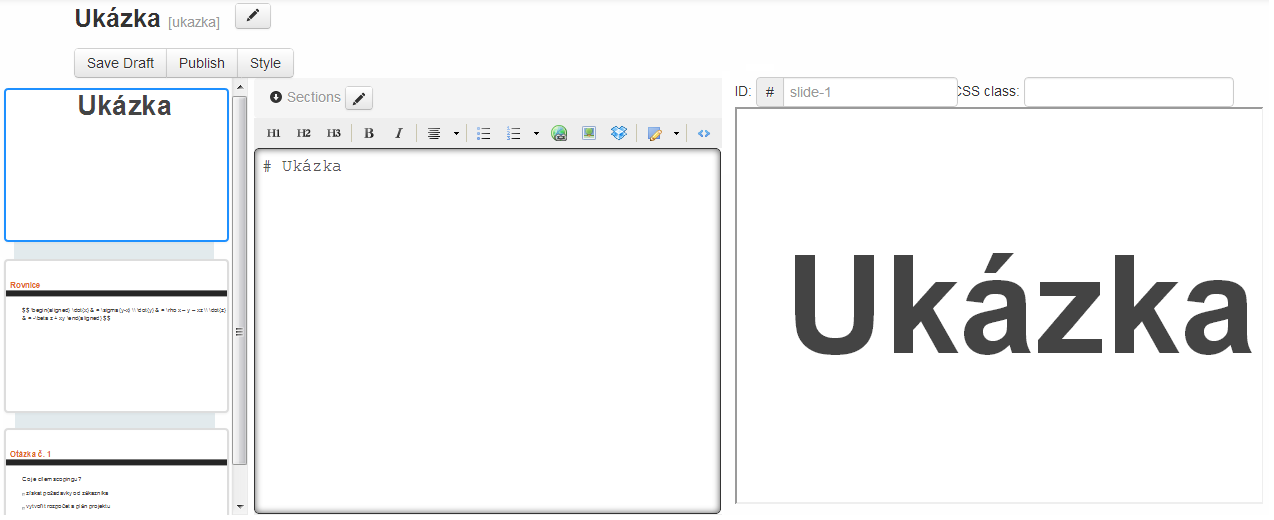
\includegraphics[width=14cm]{PRO-img/editor2.png}
		\caption{Ukázka editoru}
		\label{fig:editorLayout}
	\end{center}
\end{figure}


\section{Chování editoru}
V následujícím textu je popsáno, jak editor prezentace funguje.

Při načtení stránky editoru se obsah prezentace převede na JavaScriptový objekt, který uchovává informace o jednotlivých snímcích. Součástí těchto dat je zdrojový text obsahu snímku a také jeho HTML podoba po konverzi. HTML kód každého snímku se pak vloží do panelu s~malými náhledy. Malý náhled snímku je pomocí CSS pravidel zmenšen, jinak by obsah byl stejně velký jako v~normálním zobrazení prezentace.

Po kliknutí na malý náhled se objeví v~textovém poli pro úpravu snímku zdrojový text snímku a ve velkém náhledu vpravo se objeví kompletní snímek s~inicializovanou knihovnou deck.js, tj. včetně funkční interakce.

Při změně zdrojového textu snímku se celý obsah automaticky posílá na server, kde se text pomocí knihovny Texy! převádí na HTML kód. Výsledný HTML kód snímku se následně vrací v odpovědi. Poté se aktualizují oba náhledy snímku, malý i velký. Aby se ale na server neposílala každá úprava snímku (např. po stisku každého písmene), a tak nevhodně zatěžovala server i klientskou aplikaci, byla implementovaná čekací doba 1 sekundy. Pokud po poslední změně snímku uplyne tato doba, během které nebyla provedena žádná další úprava, pošle se požadavek na převod zdrojového textu na server.


\section{Úprava knihovny Texy!}
Následující odstavce popisují rozšíření jednoduchého značkovacího jazyka Texy!. Bylo totiž nutné vymyslet a implementovat novou syntaxi pro interaktivní odpovídání na kvizové otázky během prezentace a další novinky. Dále jsem se pokusil upravit syntaxi značkovacího jazyka Texy! pro lepší kompatibilitu s více rozšířeným a známým jazykem Markdown.

\subsection{Markdown syntaxe}
Jak už bylo vysvětleno v předchozích kapitolách, pro popis snímků byla použita knihovna Texy!, která implementuje vlastní jazyk stejného jména. Tento jazyk je ovšem široce používaný pouze v českých a slovenských zemích. Celosvětově ho zastiňuje mnohem více rozšířený značkovací jazyk Markdown. Oba jazyky jsou si v lecčem podobné, avšak najdou se i velké rozdíly. Proto jsem se rozhodl knihovnu Texy! upravit a některé části přizpůsobit syntaxi jazyku Markdown.

Jeden z~nejvíce patrných rozdílů byl v~syntaxi nadpisů. Porovnejte rozdíly mezi výpisy \ref{lst:nadpisy1} a \ref{lst:nadpisy2}.

\begin{lstlisting}[caption=Ukázka nadpisů v Texy!,label={lst:nadpisy1}]
### Nadpis 1. úrovně
## Nadpis 2. úrovně
# Nadpis 3. úrovně

nebo alternativně

Nadpis 1. úrovně
################

Nadpis 2. úrovně
****************

Nadpis 3. úrovně
================
\end{lstlisting}

\begin{lstlisting}[caption=Ukázka nadpisů v Markdown,label={lst:nadpisy2}]
# Nadpis 1. úrovně
## Nadpis 2. úrovně
### Nadpis 3. úrovně

nebo alternativně

Nadpis 1. úrovně
================

Nadpis 2. úrovně
----------------
\end{lstlisting}

Jak je vidět, logika syntaxí značek u varianty před nadpisem je u obou jazyků přesně opačná. Proto byla syntaxe upravena, aby byla ekvivalentní s jazykem Markdown. Změna pak byla otestována pomocí jednotkových testů.

Protože ale sjednocení syntaxí nebylo prioritou tohoto projektu, nezaměřoval jsem se více na další zvýšení kompatibility.


\subsection{Nová syntaxe}
Dále bylo nutné rozšířit knihovnu Texy! a implementovat vlastní pravidla konverze textu do HTML. Rozšíření se týkalo možnosti uživatele odpovídat na otázky během prohlížení prezentace a dále vytvoření osnovy prezentace s odkazy na snímky.

\subsubsection{Syntaxe odpovědí}
Pro vytvoření kvizových otázek bylo potřeba vymyslet a implementovat syntaxi na vložení zaškrtávacího pole, které uživatel při prohlížení prezentace může zaškrtnout jako správnou odpověď na otázku položenou na snímku. Správných odpovědí může být více. Po delší úvaze bylo rozhodnuto, že na jednom snímku lze mít pouze jednu otázku. Nejenže by se více otázek na snímek nevešlo, ale zjednodušila se tak i složitost syntaxe, která by na tento případ musela brát ohled. Stejně tak odpadla potřeba manuálně vkládat potvrzovací tlačítko pro kontrolu zaškrtnutých odpovědí. Tlačítko se při překladu vkládá na konec snímku automaticky, pokud je na snímku použita syntaxe pro vložení zaškrtávacích políček. Ukázku syntaxe můžete vidět ve výpisu \ref{lst:odpovedi} a snímek po převodu do HTML na obrázku \ref{fig:odpovedi}.

\begin{lstlisting}[caption={Ukázka zdrojového textu snímku s otázkou a odpovědmi},label={lst:odpovedi}]
## Otázka č. 1

Co je cílem scopingu?

[+] získat požadavky od zákazníka

[-] vytvořit rozpočet a plán projektu
\end{lstlisting}


\begin{figure}[ht]
	\begin{center}
		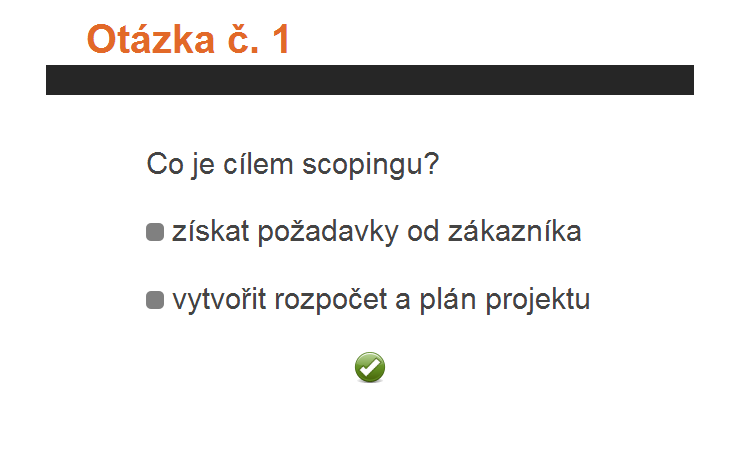
\includegraphics[width=14cm]{PRO-img/odpovedi.png}
		\caption{Ukázka snímku z otázkou a odpovědmi}
		\label{fig:odpovedi}
	\end{center}
\end{figure}

Pro vyhodnocení správnosti zaškrtnutých odpovědí musí uživatel stisknout tlačítko pro kontrolu. Případné chybné odpovědi mají za následek přiřazení CSS třídy ke špatně zaškrtnutým políčkům.

Samotná zaškrtávací políčka nejsou zobrazena jako HTML vstupní pole \verb|<input>| proto, aby se daly lépe vzhledově upravit pomocí CSS stylů.

\subsubsection{Syntaxe doplňkových textů}
Důležitou součástí požadovaného kvizového systému byla také možnost vkládat doplňkový text. Autor prezentace tak může uvést bližší informace k~odpovědím na danou otázku nebo odkázat na jiný snímek prezentace či dokonce na jiný web.

Tento text se rozděluje na dva typy: pro správně a nesprávně zaškrtnuté odpovědi. Tento doplňkový text se dynamicky objeví až po kliknutí na potvrzovací tlačítko, přitom text pro správně zaškrtnuté odpovědi se zobrazí při zaškrtnutí pouze správných odpovědí, u textu pro špatné odpovědi přesně naopak.

Pro vložení takového bloku textu byla použita podobná syntaxe jako pro ostatní účelové bloky textu v~syntaxi Texy!
(např. blok kódu). Použití syntaxe pro oba doplňkové texty vidíte ve výpisu \ref{lst:texts}

\begin{lstlisting}[caption={Syntaxe doplňkových textů},label={lst:texts}]
/--correct
Tento text se zobrazí při **správné** odpovědi.
\--

/--incorrect
Tento text se zobrazí při **špatné** odpovědi.
\--
\end{lstlisting}

\subsubsection{Syntaxe pro vložení osnovy}
V mnoha prezentacích se můžeme setkat s více tématy nebo podtématy, o kterých prezentace pojednává. Proto editor prezentace poskytuje možnost rozdělit prezentaci na logické celky. U každého snímku tak lze specifikovat až tři úrovně sekcí, do kterých snímek logicky patří. Toho pak bylo využito pro další vlastnost převodu zdrojového textu do HTML - generování osnovy (obsahu) prezentace s odkazy na snímky, které tyto sekce specifikují. Syntaxe je pak jednoduchá, stačí uvést \verb|{table of contents}|. Při převodu je pak tato direktiva nahrazena HTML seznamem sekcí a případných podsekcí s odkazy vedoucími na dané snímky.


\section{Rozšíření prezentační knihovny}
Protože tento nástroj byl zaměřen na použití ve vzdělávacích institucích, bylo dobrou myšlenkou rozšířit možnosti prezentační knihovny o další pomocné funkce. Rozhodl jsem se proto implementovat funkci zvýraznění syntaxe bloků programovacích jazyků, která se určitě bude hodit prezentujícím vývojářům, a dále zobrazení matematických vzorců ve formátu \LaTeX, které bude možné použít například v prezentacích z oboru matematiky.

\subsection{Zvýraznění syntaxe programovacích jazyků}
Pro zobrazení kódu používá knihovna Texy! blokovou syntaxi jakou můžete vidět ve výpisu \ref{lst:code}. Po převodu tohoto textu do HTML se uvedený kus kódu obalí do sebe vnořených sémantických HTML značek \verb|<pre>| a \verb|<code>|. Toho je pak využito při zvýraznění syntaxe, jež je zajištěno pomocí knihovny highlight.js\cite{highlight}, která automaticky tyto bloky kódu za použití detekce jazyka zvýrazní. Knihovna podporuje více než 50 jazyků.

\begin{lstlisting}[caption={Ukázka blokové syntaxe pro výpis kódu},label={lst:code}]
/--code
SELECT * FROM `presentations` where `id` = 1;
\--
\end{lstlisting}


\subsection{Matematické vzorce}
Další přidanou hodnotou do prohlížení prezentací bylo zavedení zobrazení matematických vzorců a rovnic. Není totiž nijak uživatelsky příjemné tyto vzorce vytvářet jako obrázky a vkládat je pak do prezentace. Pro implementaci této vlastnosti byla použita JavaScriptová knihovna MathJax\citep{mathjax}, která automaticky vyhledává zdrojový text ve formátu \LaTeX\cite{latex} ve specifické syntaxi a následně je vysází pomocí HTML a CSS za použití webových fontů. Není tedy potřeba žádných dalších technologií třetích stran, jako například Flash, a zároveň se nejedná o obrázky, zachovává si tak všechny vlastnosti okolního textu, jako barva či velikost.

Podmínkou pro vyhledání a zobrazení vzorců je ohraničení zdrojového textu vzorců oddělovači. Ty jsou dvojího druhu, protože knihovna podporuje zobrazení jak blokových vzorců, tak tzv. inline vzorců, ty mohou být součástí odstavců textu. Oddělovače pro inline vzorce jsou \verb|$(| a \verb|)$|, pro blokové vzorce pak \verb|$$| a \verb|$$|. Ukázku použití této syntaxe spolu se vzorovým zdrojovým textem několika rovnic vidíte ve výpisu \ref{lst:rovnice}, výsledný snímek s vysázenými matematickými rovnicemi vidíte na obrázku \ref{fig:rovnice}.

\begin{lstlisting}[caption={Ukázka syntaxe matematických vzorců},label={lst:rovnice}]
## Rovnice

$$
\begin{aligned}
\dot{x} & = \sigma(y-x) \\
\dot{y} & = \rho x - y - xz \\
\dot{z} & = -\beta z + xy
\end{aligned}
$$
\end{lstlisting}

\begin{figure}[ht]
	\begin{center}
		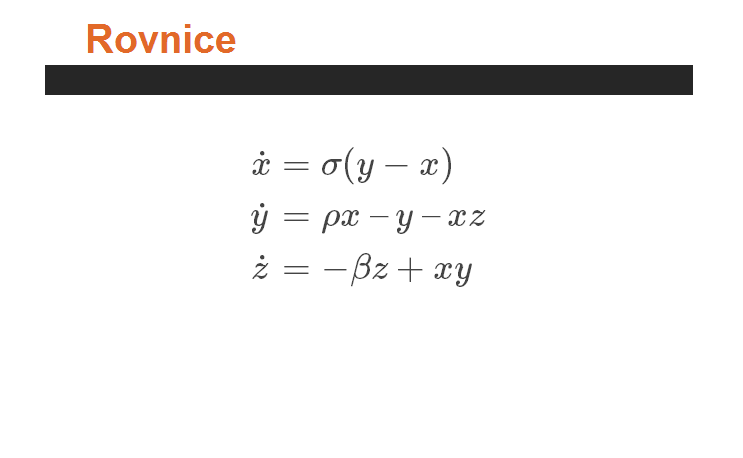
\includegraphics[width=14cm]{PRO-img/rovnice.png}
		\caption{Ukázka snímku s matematickými rovnicemi}
		\label{fig:rovnice}
	\end{center}
\end{figure}



\chapter{Nasazení}

\section{Server}
Pro chod systému je nutný spuštěný webový server, na kterém běží PHP a databáze MySQL. Pro vývoj používám hotové řešení WAMP (Windows, Apache, MySQL, PHP) jménem EasyPHP. Verze komponent:

\begin{itemize}
	\item Apache 2.2
	\item PHP 5.3
	\item MySQL 5.5
\end{itemize}

Pro nasazení na produkční prostředí jsem se rozhodl využít cloudového systému PHP Fog\footnote{\url{http://phpfog.com}}. Pro malý počet aplikací a malý rozsah poskytuje své služby zdarma. V placených řešení je pak největší výhodou možnost škálování instancí aplikace či paměti nebo velké množství rozšíření (např. analytické nástroje či optimalizační nástroje pro databázi). Server uchovává aplikaci jako git repozitář a tak pro nahrání nové verze aplikace stačí příkaz push.

V listopadu 2012 bylo ovšem oznámeno ukončení provozu PHP Fogu a postupné odpojování bezplatných aplikací v průběhu prosince. Jako náhrada byla doporučena podobná služba AppFog\footnote{\url{http://www.appfog.com/}} od stejné firmy.



\chapter{Shrnutí}
Projekt byl velmi zajímavý. Vyzkoušel jsem si několik nových technologií, zejména AngularJS, který určitě budu dál sledovat a snad s~ním i někdy znovu pracovat. Opět jsem ale došel k~závěru, že zkoumání a použití nových a neznámých vlastností v~technologiích HTML(5) není jednoduché a bezproblémové.

Jsem rád, že jsem použil Nette framework, který dobře znám a tak jsem neměl tolik problémů u~serverové části. Ze začátku jsem se ovšem rozhodoval, jestli si nevyzkoušet nějakou jinou technologii, například dnes moderní Ruby on Rails nebo Node.js. Mohu ale říct, že bych si nepřál znovu dělat tento projekt v~jiné technologii, neboť by mi to přineslo o to více problémů.

Více práce by si rozhodně zasloužila podoba editoru a obecná uživatelská přívětivost. Jinak ale výsledek projektu hodnotím kladně.




\bibliographystyle{csplainnat}
{
\def\CS{$\cal C\kern-0.1667em\lower.5ex\hbox{$\cal S$}\kern-0.075em $}
\bibliography{BP-ref}
}




%%%%%%%%%%%%%%%%%%%%%%%%%% 
% vše co následuje bude uvedeno v přílohách
\appendix	

\printnomenclature


\chapter{Obsah přiloženého CD}

%\begin{figure}[h]
%\begin{center}
%\includegraphics[width=14cm]{figures/seznamcd}
%\caption{Seznam přiloženého CD --- příklad}
%\label{fig:seznamcd}
%\end{center}
%\end{figure}



\end{document}

















